\documentclass[tikz,border=14pt]{standalone}
\usepackage[T1]{fontenc}
\usepackage{tgheros}
\usepackage{sfmath}
\usepackage{amsmath}
% % \usepackage{fontawesome5} (Removed for publication-grade academic typography) (Removed for publication-grade academic typography)
\usepackage{tikz}
\usetikzlibrary{arrows.meta,positioning,shapes.geometric,fit,backgrounds,calc}
\usepackage{xcolor}

\renewcommand{\familydefault}{\sfdefault}

% Harvard Crimson & ETH Zurich Academic Semantic Palette
\definecolor{harvardcrimson}{HTML}{A51C30}
\definecolor{ethdarkblue}{HTML}{1F407A}
\definecolor{ethblue}{HTML}{215CAF}
\definecolor{ethpetrol}{HTML}{007A87}
\definecolor{ethbronze}{HTML}{B87333}
\definecolor{ethpurple}{HTML}{5B4B8A}
\definecolor{ethslate}{HTML}{475569}
\definecolor{cardbg}{HTML}{F8FAFC}
\definecolor{cardborder}{HTML}{CBD5E1}
\definecolor{safeTeal}{HTML}{10B981}

\begin{document}
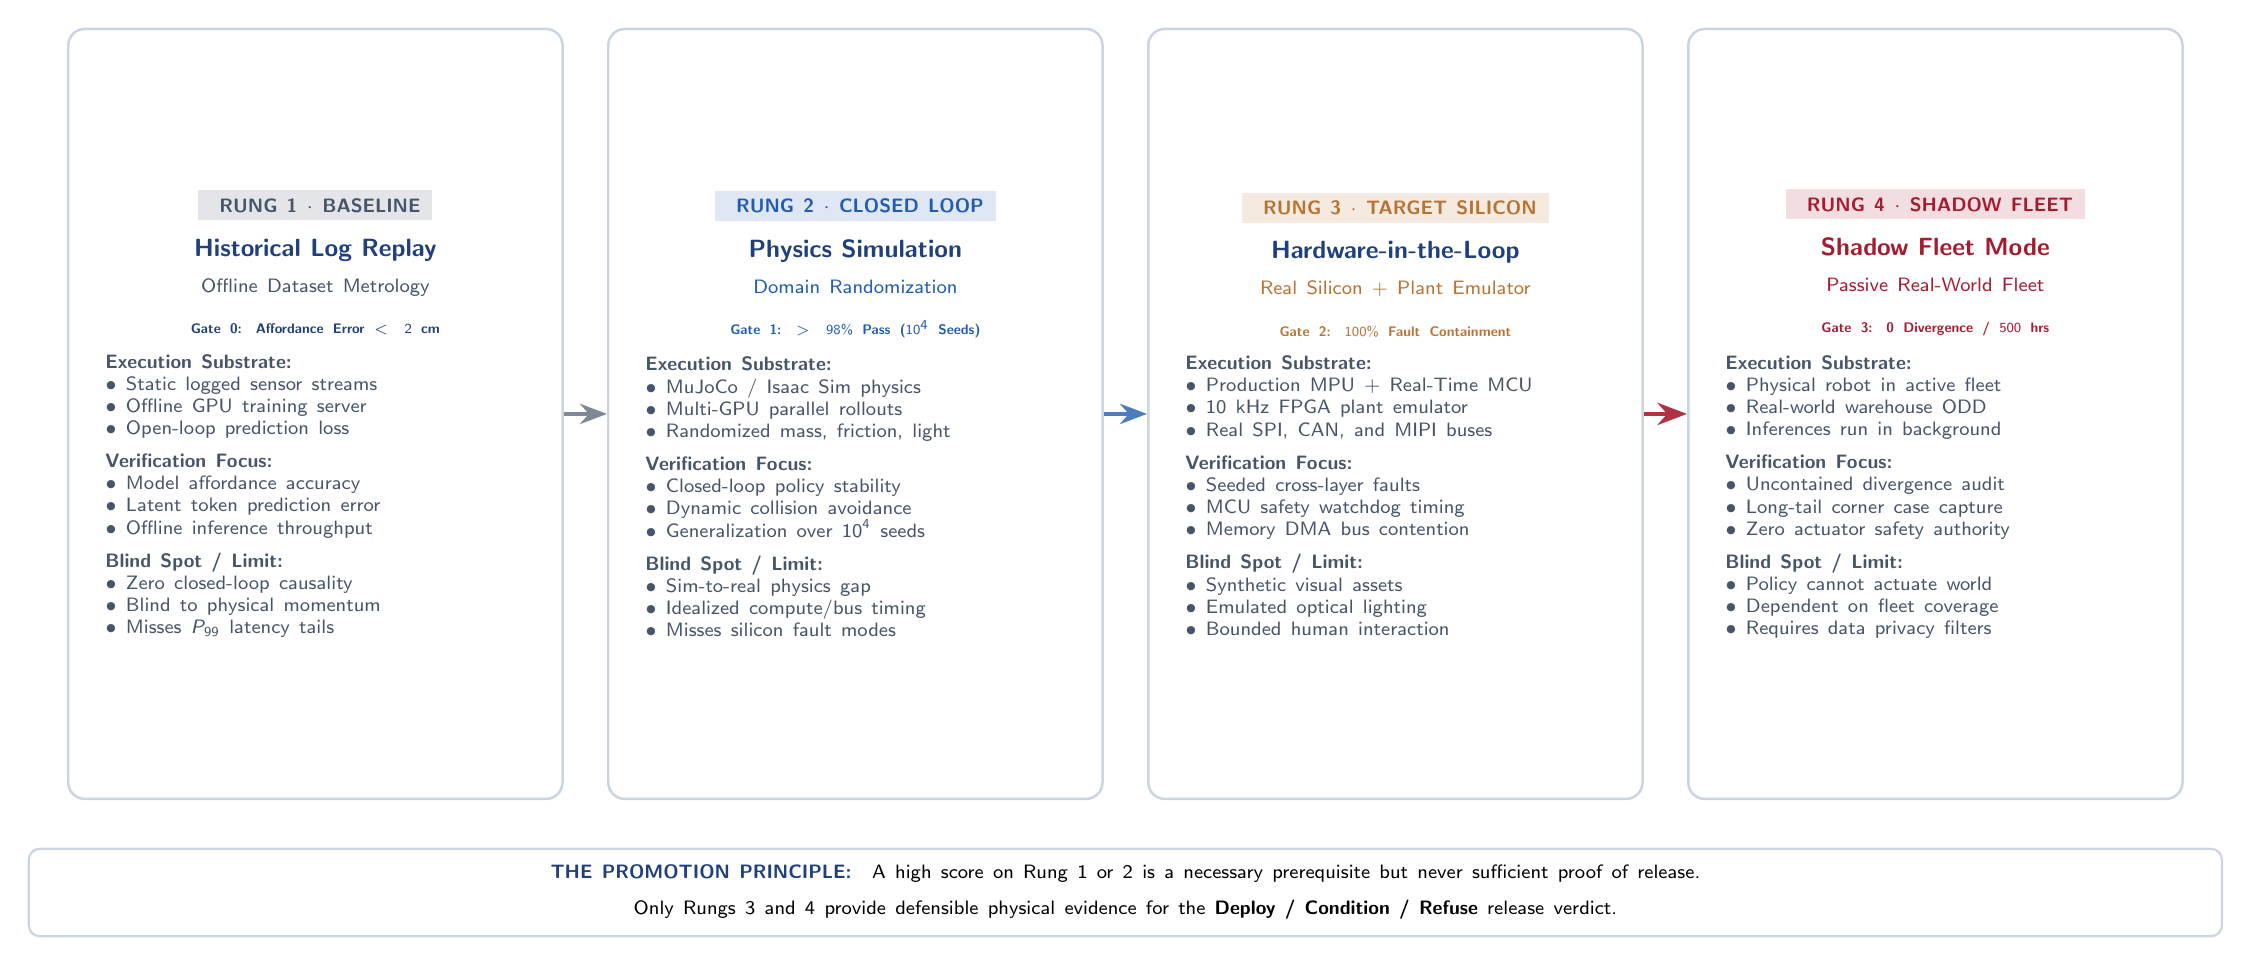
\begin{tikzpicture}[
  font=\sffamily,
  >=Stealth,
  laddercard/.style={
    draw=cardborder,
    fill=white,
    rounded corners=6pt,
    line width=0.9pt,
    text width=2.25in,
    minimum height=3.85in,
    inner sep=8pt,
    align=center,
    anchor=north
  }
]

  % Top Title Banner
  % (Top title banner removed for academic publication standards)
% --- RUNG 1: HISTORICAL LOG REPLAY ---
  \node[laddercard] (r1) at (1.25in, 0.00in) {
    {\scriptsize\bfseries\color{ethslate}\colorbox{ethslate!15}{\, RUNG 1 $\cdot$ BASELINE\,}}\\[4pt]
    {\small\bfseries\color{ethdarkblue}Historical Log Replay}\\[1pt]
    {\scriptsize\color{ethslate}Offline Dataset Metrology}\\[3pt]
    {\tiny\bfseries\color{ethdarkblue} Gate 0: Affordance Error $< 2\text{ cm}$}\\[6pt]
    \begin{minipage}{2.10in}
    \scriptsize\raggedright\color{ethslate}
    \textbf{Execution Substrate:}\\
    $\bullet$ Static logged sensor streams\\
    $\bullet$ Offline GPU training server\\
    $\bullet$ Open-loop prediction loss\\[4pt]
    \textbf{Verification Focus:}\\
    $\bullet$ Model affordance accuracy\\
    $\bullet$ Latent token prediction error\\
    $\bullet$ Offline inference throughput\\[4pt]
    \textbf{Blind Spot / Limit:}\\
    $\bullet$ Zero closed-loop causality\\
    $\bullet$ Blind to physical momentum\\
    $\bullet$ Misses $P_{99}$ latency tails
    \end{minipage}
  };

  % --- RUNG 2: DOMAIN-RANDOMIZED SIMULATION ---
  \node[laddercard] (r2) at (3.95in, 0.00in) {
    {\scriptsize\bfseries\color{ethblue}\colorbox{ethblue!15}{\, RUNG 2 $\cdot$ CLOSED LOOP\,}}\\[4pt]
    {\small\bfseries\color{ethdarkblue}Physics Simulation}\\[1pt]
    {\scriptsize\color{ethblue}Domain Randomization}\\[3pt]
    {\tiny\bfseries\color{ethblue} Gate 1: $> 98\%$ Pass ($10^4$ Seeds)}\\[6pt]
    \begin{minipage}{2.10in}
    \scriptsize\raggedright\color{ethslate}
    \textbf{Execution Substrate:}\\
    $\bullet$ \mbox{MuJoCo} / \mbox{Isaac Sim} physics\\
    $\bullet$ Multi-GPU parallel rollouts\\
    $\bullet$ Randomized mass, friction, light\\[4pt]
    \textbf{Verification Focus:}\\
    $\bullet$ Closed-loop policy stability\\
    $\bullet$ Dynamic collision avoidance\\
    $\bullet$ Generalization over $10^4$ seeds\\[4pt]
    \textbf{Blind Spot / Limit:}\\
    $\bullet$ Sim-to-real physics gap\\
    $\bullet$ Idealized compute/bus timing\\
    $\bullet$ Misses silicon fault modes
    \end{minipage}
  };

  % --- RUNG 3: HARDWARE-IN-THE-LOOP (HIL) ---
  \node[laddercard] (r3) at (6.65in, 0.00in) {
    {\scriptsize\bfseries\color{ethbronze}\colorbox{ethbronze!15}{\, RUNG 3 $\cdot$ TARGET SILICON\,}}\\[4pt]
    {\small\bfseries\color{ethdarkblue}Hardware-in-the-Loop}\\[1pt]
    {\scriptsize\color{ethbronze}Real Silicon + Plant Emulator}\\[3pt]
    {\tiny\bfseries\color{ethbronze} Gate 2: $100\%$ Fault Containment}\\[6pt]
    \begin{minipage}{2.10in}
    \scriptsize\raggedright\color{ethslate}
    \textbf{Execution Substrate:}\\
    $\bullet$ Production MPU + Real-Time MCU\\
    $\bullet$ $10\text{ kHz}$ FPGA plant emulator\\
    $\bullet$ Real SPI, CAN, and MIPI buses\\[4pt]
    \textbf{Verification Focus:}\\
    $\bullet$ Seeded cross-layer faults\\
    $\bullet$ MCU safety watchdog timing\\
    $\bullet$ Memory DMA bus contention\\[4pt]
    \textbf{Blind Spot / Limit:}\\
    $\bullet$ Synthetic visual assets\\
    $\bullet$ Emulated optical lighting\\
    $\bullet$ Bounded human interaction
    \end{minipage}
  };

  % --- RUNG 4: SHADOW FLEET DEPLOYMENT ---
  \node[laddercard] (r4) at (9.35in, 0.00in) {
    {\scriptsize\bfseries\color{harvardcrimson}\colorbox{harvardcrimson!15}{\, RUNG 4 $\cdot$ SHADOW FLEET\,}}\\[4pt]
    {\small\bfseries\color{harvardcrimson}Shadow Fleet Mode}\\[1pt]
    {\scriptsize\color{harvardcrimson}Passive Real-World Fleet}\\[3pt]
    {\tiny\bfseries\color{harvardcrimson} Gate 3: 0 Divergence / $500\text{ hrs}$}\\[6pt]
    \begin{minipage}{2.10in}
    \scriptsize\raggedright\color{ethslate}
    \textbf{Execution Substrate:}\\
    $\bullet$ Physical robot in active fleet\\
    $\bullet$ Real-world warehouse ODD\\
    $\bullet$ Inferences run in background\\[4pt]
    \textbf{Verification Focus:}\\
    $\bullet$ Uncontained divergence audit\\
    $\bullet$ Long-tail corner case capture\\
    $\bullet$ Zero actuator safety authority\\[4pt]
    \textbf{Blind Spot / Limit:}\\
    $\bullet$ Policy cannot actuate world\\
    $\bullet$ Dependent on fleet coverage\\
    $\bullet$ Requires data privacy filters
    \end{minipage}
  };

  % Clean Un-Occluded Promotion Arrows Between Rungs
  \draw[->, line width=1.5pt, ethslate!70] (r1.east) -- (r2.west);
  \draw[->, line width=1.5pt, ethblue!80] (r2.east) -- (r3.west);
  \draw[->, line width=1.7pt, harvardcrimson!90] (r3.east) -- (r4.west);

  % Bottom Summary Strip
  \node[draw=cardborder, fill=white, rounded corners=4pt, line width=0.8pt, text width=10.80in, inner sep=6pt, anchor=north, align=center] 
    at (5.30in, -4.10in) {
    {\scriptsize\textbf{\color{ethdarkblue} THE PROMOTION PRINCIPLE:}\;\; A high score on Rung 1 or 2 is a necessary prerequisite but never sufficient proof of release.\\[1pt]
    Only Rungs 3 and 4 provide defensible physical evidence for the \textbf{Deploy / Condition / Refuse} release verdict.}
  };

\end{tikzpicture}
\end{document}
